\documentclass[finnish,colorlinks]{scrartcl}

\usepackage[utf8]{inputenc}
\usepackage[T1]{fontenc}
\usepackage{libertine}
\usepackage{babel}
\usepackage{graphicx}
\usepackage{hyperref}

\urlstyle{same}

\begin{document}
\subject{Web"-palvelinohjelmointi Java "=kurssin harjoitustyö}
\title{insta}
\subtitle{Versio 0.9}
\author{Janne Suomalainen}
\maketitle
\tableofcontents
\section{Sovellus}
Sovellus löytyy osoitteesta \url{https://evening-island-18993.herokuapp.com}. Sovelluksen lähdekoodi löytyy \href{https://github.com/suomja1/insta}{GitHubista} ja sen testaus\footnote{Versiossa 0.9 ei ole implementoitu yhtään testiä.} on automatisoitu \href{https://travis-ci.org/suomja1/insta}{Travis-palvelun} avulla.
\subsection{Kuvaus}
\subsection{Profiilit}
\subsection{Tunnistautuminen}
\subsection{Tietokantakaavio}
Sovellus käyttää tietokantaa, jossa on yhteensä viisi taulua. Yksi näistä on liitostaulu. Tietokantakaavio on esitetty kuvassa~\ref{fig:tk}.

\begin{figure}[ht]
\centering
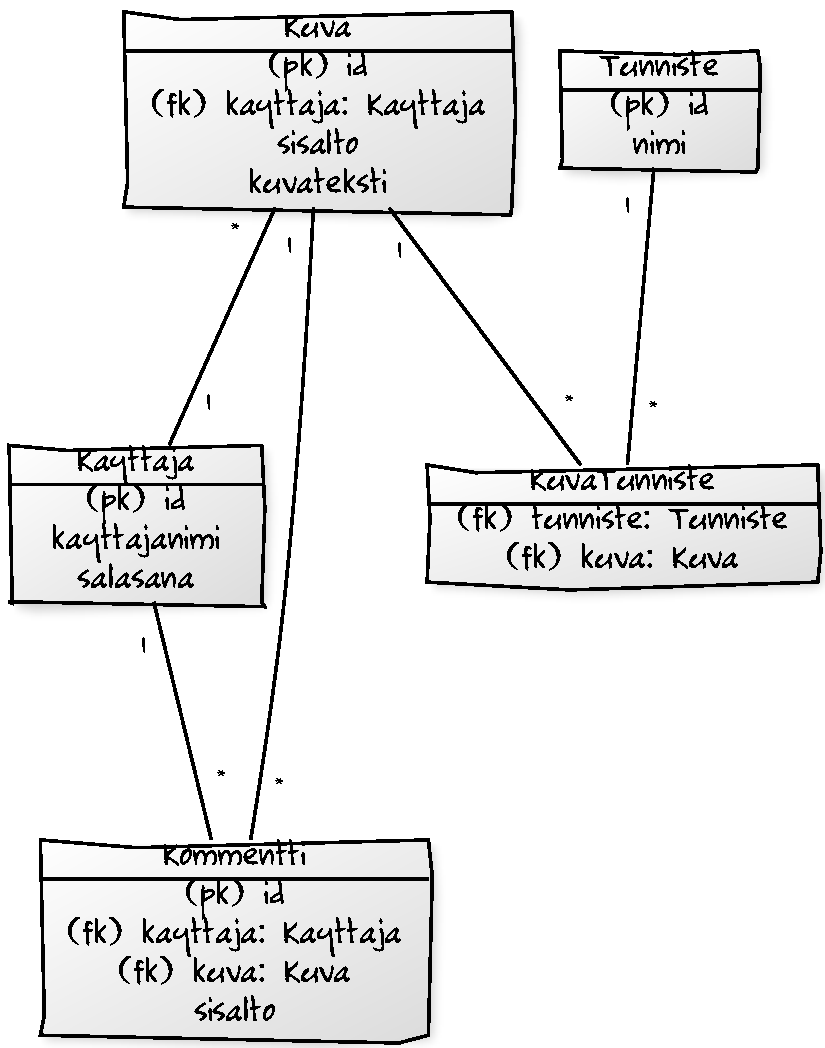
\includegraphics[width=.5\linewidth]{6424b8c7}
\caption{Tietokantakaavio.}\label{fig:tk}
\end{figure}
\section{Keskeisiä käyttötapauksia}
\subsection{Syötteiden validointi}
\section{Jatkokehitys}
testit

syötteiden validointi

roolit

virheviestit
\end{document}